\chapter{Ausgangssituation}
\section{Projektteam}
Das Projektteam besteht aus drei Schülern des Linzer Technikums, der Abteilung
Informationstechnologie.

\vspace{1cm}
\begin{table}[htbp]
  \centering
  \begin{tabular}{ccc}
    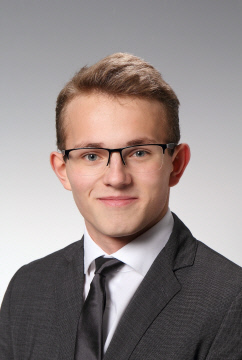
\includegraphics[width=0.3\textwidth]{FLUTTER/images/Grubauer_Patrick.jpg} &
    % 
\includegraphics[width=0.31925\textwidth]{FLUTTER/images/Mayrhofer_Johannes-min.jpg} &
    
\includegraphics[width=0.3\textwidth]{FLUTTER/images/Mayrhofer_Johannes_2.jpg} &
    \includegraphics[width=0.3\textwidth]{FLUTTER/images/Zöchmann_Benedikt.jpg} \\
    Patrick Grubauer &
    Johannes Mayrhofer &
    Benedikt Zöchmann \\
  \end{tabular}
  \label{tab:example}
\end{table}

\newpage

\section{Problemstellung}
Der Kartenverleih für Drucker Karten an der Schule, die für Schularbeiten und Tests oder bei der Abhaltung der Matura benötigt werden, wird derzeit mittels Eintragung in einer Liste umgesetzt. Dadurch ist die Ausleihe und die Rückgabe der Karten an die Anwesenheit von Kollegen in einem bestimmten Raum gebunden. Um in Zukunft einen orts- und zeitungebundenen Ausleihprozess zu gewährleisten, arbeiten zwei Diplomarbeiten der Informationstechnologie bzw. Mechatronik-Abteilung an einer innovativen Lösung. Die vorliegende Arbeit beschäftigt sich schwerpunktmäßig mit der softwaretechnischen Umsetzung.

\section{Arbeitsaufteilung}
\begin{itemize}
    \item Johannes Mayrhofer: \\ Zentrale Schnittstelle: Client -- Server -- Schließfach -- Hardware Kommunikation\\ Datenbank \\ Simulation des Gesamtsystems
    \item Patrick Grubauer: Flutter App $\rightarrow$ Client – Sicht, Login – Sicht, Display – Sicht.
    \item Benedikt Zöchmann: Flutter App $\rightarrow$ Admin – Sicht.
\end{itemize}

% \newpage

